\chapter{O número de Helly e o número de Helly forte para grafos $B_k$-EPG e $B_k$-VPG}


\begin{flushright}
\begin{minipage}[t][0cm][b]{0.47\textwidth}
\emph{
%A Matemática é o alfabeto com o qual Deus escreveu o Universo.
Falta algo para completar esta demonstração, mas não tenho tempo.}
\end{minipage}

\rule[0cm]{7cm}{0.03cm}%{largura}{espessura}

Évariste Galois
\end{flushright}




O estudo de grafos EPG foi introduzido por  Golumbic, Lypshteyn e Stern (2009) e consiste dos grafos de intersecção de conjuntos de caminhos sobre uma grade ortogonal, cujas intersecções são tomadas considerando as arestas dos caminhos. Se as intersecções dos caminhos consideram os vértices e não as arestas, a classe de grafos resultante é chamada de grafos VPG. Tal classe foi introduzida em 2011 \cite{asinowski2011string} e \cite{asinowski2012}. Nesse capítulo estudaremos dois parâmetros em ambas classes de grafos EPG e VPG. Os parâmetros que serão estudados são nomeadamente o número de Helly e o número de Helly forte.

\section{Discussão Inicial}

Seja  $\cal {F}$ uma família de conjuntos de algum conjunto universal $U$, e $h$ um número inteiro tal que $h\geq 1$. Podemos dizer que $\cal{F}$ é $h$-{\it intersectante} quando todos  $h$ subconjuntos de $\cal {F}$ intersectam-se. Chamamos de {\it core} de $\cal {F}$ a intersecção de todos conjuntos de $\cal {F}$, e denotamos por $core(\cal F)$. 

A família $\cal{F}$ é $h$-{\it Helly} quando toda subfamília $h$-intersectante $\cal{F'}$ satisfaz $core(\cal{F'}) \neq \emptyset$, ver mais em \cite{duchet1978propriete}. Por outro lado, se para toda subfamília $\cal{F'}$ de $\cal{F}$, existem $h$ subconjuntos cujo core é igual ao core de  $\cal {F'}$, então $\cal {F}$ é dito ser  $h$-{\it Helly} {\it forte}. Claramente, se $\cal {F}$ é $h$-Helly então ele também é $h'$-Helly, para $h' \geq h$. Similarmente, se ${\cal F}$ é $h$-Helly forte então ele também é $h'$-Helly forte, para $h' \geq h$. 

Finalmente, o   {\it número de Helly} da família  $\cal{F}$ é o menor inteiro $h$, tal que $\cal{F}$ é  $h$-Helly. Similarmente, o {\it número de Helly forte} de  $\cal{F}$ é o menor $h$, para o qual  $\cal{F}$ é  $h$-Helly forte. Também segue que o número de Helly forte de $\cal{F}$ é no mínimo igual ao seu número de Helly.


Uma  {\it classe} $\cal {C}$ de famílias $\cal {F}$  de subconjuntos de algum conjunto universal $U$ é uma  subcoleção das famílias $\cal {F}$ de $U$. Dizemos que  $\cal C$ é uma {\it classe hereditária}, quando ela é fechada sob inclusão, i.e. se um grafo $G$ pertence a uma classe $C$ então todo subgrafo induzido de $G$ também pertence a $C$. O {\it número de Helly}  de uma classe  $\cal{C}$ de famílias $\cal{F}$ de subconjuntos é o maior número de Helly entre todas as famílias de $\cal {F}$. Similarmente, o {\it número de Helly forte} de uma classe  $\cal {C}$ é o maior número de Helly forte das famílias de $\cal {C}$.

Se $\cal F$ é uma família de subconjuntos e $\cal C$ uma classe de famílias, denotamos por $H(\cal F)$ e por 
$H(\cal C)$,  o número de  Helly de $\cal F$ e $\cal C$, respectivamente, enquanto  $sH({\cal F})$ e $sH({\cal C})$  representam os números de  Helly forte de $\cal F$ e $\cal C$.


Nesse capítulo, nos preocupamos com famílias de subconjuntos $\cal{F}$ de caminhos de arestas e vértices em uma grade. No primeiro contexto, consideramos que cada caminho $P_i$  consiste de uma sequência de arestas consecutivas na grade ortogonal, que forma o caminho, e chamaremos essas de   {\it representações EPG}. Dessa forma, segue que dois caminhos intersectam-se se e somente se eles contém no mínimo uma aresta da grade em comum. Aos grafos que  correspondem às representações EPG denotaremos por {\it grafos EPG}. 
No segundo contexto, um caminho é visto como uma sequência de vértices consecutivos, e dois caminhos intersectam-se se eles contém um vértice comum. Analogamente aos anteriores esses são chamados de {\it representações VPG} e {\it grafos VPG}. 

Cada aresta possui uma direção associada na grade, a qual pode ser horizontal ou vertical. Uma  {\it dobra} no caminho é um par de arestas consecutivas que possuem direções distintas.  Um {\it segmento} de um caminho é uma sequência de arestas consecutivas do caminho, sem dobras. Dizemos que o caminho $P_i$ é um  $B_k$-{\it path} se ele contém $k$ dobras. Dizemos que $\cal {F}$ é uma família de $B_k$-caminhos, ou simplesmente  uma $B_k$-família, se cada caminho de $\cal {F}$ contém no máximo $k$ dobras. 

 Nesse capítulo, resolvemos completamente o problema de determinar ambos o número de Helly e o número de Helly forte, para ambos contextos de grafos $B_k$-EPG e $B_k$-VPG. Determinamos o número de Helly em grafos $B_k$-EPG e $B_k$-VPG, para cada valor de $k$.

Para grafos EPG, o número de Helly de $B_0$-families é bem conhecido e é igual a 2, uma vez que  grafos $B_0$-EPG coincidem com grafos de intervalo. Também é simples concluir que o número de Helly forte dos grafos $B_0$-EPG é também igual a 2. Para $k = 1$,   provamos que ambos o número de Helly e número de Helly forte da classe de $B_1$-families são iguais a 3. Para a classe de  $B_2$-families, provamos que esses dois parâmetros são iguais a 4. Além disso o número de Helly e número de Helly forte para $B_3$-families é igual a 8, e finalmente esses parâmetros são ilimitados para  $k \geq 4$. 
Quanto aos grafos VPG, é simples concluir que o número de Helly de grafos $B_0$-VPG é igual a 2, e provamos que grafos $B_1$-VPG possuem número de Helly  4, grafos $B_2$-VPG possuem número de Helly  6, grafos $B_3$-VPG possuem número de Helly 12, enquanto o número de Helly para grafos $B_4$-VPG novamente é ilimitado.

Finalmente, o número de Helly forte é igual ao número de Helly nos grafos  $B_k$-EPG, para cada $k$. O mesmo vale para grafos $B_k$-VPG.

Com relação aos resultados existentes, 
Golumbic, Lipshteyn  e Stern \cite{golumbic2009} já tem mostrado que o número de Helly forte para grafos $B_1$-EPG é igual a 3, e para grafos $B_1$-VPG é igual a  4. Empregando técnicas de prova diferentes das utilizadas neste trabalho. Veja  \cite{golumbic2019edge}, Teorema 11.13, abaixo:
\begin{theorem}\label{thm:golumbic2019edge}{\cite{golumbic2019edge}}
Seja $P$ uma coleção de caminhos de dobra simples sobre uma grade. Se cada 2 caminhos em  $P$ compartilham no mínimo uma aresta da grade, então $P$ possui número de Helly forte igual a 3. Caso contrário, $P$ possui número de Helly forte igual a 4. 
\end{theorem}
Nenhum outro resultado relacionado ao número de Helly forte, ou resultados relacionados ao número de Helly de grafos $B_k$-EPG foi notado ter sido reportado na literatura levantada. Quanto a outras classes, Golumbic e Jamison  tem determinado o número de Helly forte dos caminhos de intersecção de arestas sobre uma árvore em~\cite{golumbic1985}. Finalmente, Asinowski, Cohen, Golumbic, Limouzy, Lipshteyn e Stern tem reportado que o número de Helly forte de grafos $B_0$-VPG é igual a 2 \cite{asinowski2011string}.  
Alguns resultados relacionados estão listados a seguir. Decidir se um dado hipergrafo é  $k$-Helly pode ser feito em tempo polinomial para um  $k$ fixo,  empregando a caracterização proposta por Berge e Duchet \cite{bergeDuchet1975}. Para algum $k$ arbitrário, o problema é  \cal{co-NP}-completo \cite{dourado2009}. Para ver mais problemas correspondendo à propriedade $k$-Helly forte e exemplos sugerimos a leitura de~\cite{dourado2008strong,dourado2009}.

Este capítulo está organizado como listado a seguir. A seção~\ref{sec:preliminares4}, contém algumas proposições preliminares e notações adicionais utilizadas neste escrito. A seção~\ref{sec:Helly-number}  descreve os resultados para o número de Helly de grafos $B_k$-EPG, enquanto a seção~\ref{sec:helly-vpg} contém resultados desse parâmetro para grafos $B_k$-VPG. O número de Helly forte é considerado na seção~\ref{sec:helly-forte}. Considerações finais são efetuadas na seção~\ref{sec:finalRemarks4}.

\section{Preliminares}\label{sec:preliminares4}

O seguinte teorema caracteriza famílias de subconjuntos $h$-Helly.


\begin{theorem}\label{thm:BD}(\cite{bergeDuchet1975}):
Uma família $\cal{F}$ de subconjuntos do conjunto universal  $U$ é $h$-Helly se e somente se para todo subconjunto   $U' \subseteq U$, $|U'|= h+1$,  a subfamília  $\cal{F'}$ de $\cal{F}$,  formada pelos subconjuntos contendo no mínimo  $h$ dos $h+1$ elementos de $U'$, tem um core não vazio. 
\end{theorem}

O próximo teorema é central para os nossos resultados.

\begin{theorem}\label{thm:minimal}Seja ${\cal C}$ uma classe hereditária de famílias ${\cal F}$ de subconjuntos do conjunto universal $U$, cujo número de Helly $H({\cal C})$ é igual a $h$. Então, existe uma família ${\cal F'} \in {\cal C}$ com exatamente $h$ subconjuntos, satisfazendo as seguintes condições: 

Para cada subconjunto  $P_i \in \cal {F'}$, existe exatamente um elemento distinto $u_i \in U$, tal que \\
$$u_i \not \in P_i,$$ 
mas $u_i$ está contido em todos subconjuntos 
$$P_j \in {\cal F'} \setminus P_i.$$
\end{theorem}
 

Proof: 
Seja ${\cal C}$ uma classe de famílias  ${\cal F}$ de subconjuntos $P$, cada subconjunto formado pelos elementos  $u \in U$, tal que o número de Helly $H({\cal C})$  é igual a $h$. Então cada família   ${\cal F} \in {\cal C}$ satisfaz $H({\cal F}) \leq h$. Considere uma família ${\cal F'} \in {\cal C}$  cujo número de Helly é  exatamente $h$, e contendo exatamente $h$ subconjuntos. Essa família deve existir uma vez que  ${\cal C}$ é uma classe hereditária. Além disso $H({\cal F'}) = h$, $\cal F'$ é $h$-intersectante, e portanto $(h-1)$-intersectante. Ademais, ${\cal F'}$ não é $(h-1)$-Helly. Aplicando o   Teorema~\ref{thm:BD}, podemos concluir que existem   $h$ elementos $U' = \{u_1, \ldots, u_h\} \subset U$, tal que cada conjunto de ${\cal F'}$ contem no mínimo $h-1$ elementos de $U'$. Uma vez que $H({\cal F'}) > h-1$, $core({\cal F'}) = \emptyset$ e além disso não existe elemento comum entre os conjuntos de $\cal F'$. Em particular, uma vez que cada conjunto $P_i \in {\cal F'}$ contem no mínimo  $h-1$ elementos de $U'$, e $core(\cal F') = \emptyset$, podemos escolher   $h$ subconjuntos $P_i$, em que cada um deles deixa de possuir um elemento distinto  $u_i \in U'$. Então para cada subconjunto  $P_i \in \cal F$, existe algum elemento $u_i \not \in P_i$, mas $u_i \in P_j$, para todos $P_j \in \cal F'$, $j \neq i$. \qed

Seja $\cal{ F'}$ como descrito no teorema anterior. É simples concluir que ao remover qualquer subconjunto de $\cal {F'}$ este torna-se $(h-1)$-Helly.  Todavia podemos chamar $\cal {F'}$ de uma {\it família minimal não}-$(h-1)$-{\it Helly}. Além do mais, o elemento $u_i \not \in P_i$, contido em todos os subconjuntos $P_j \in {\cal{F'}} \setminus P_i$, exceto $P_i$, é o {\it $h$-não-representativo} de $P_i$.  

Empregaremos as famílias de subconjuntos minimais citadas anteriormente, aplicadas à $B_k$-caminhos em uma grade. Note que $B_k$-caminhos em uma grade formam uma classe hereditária.

\section{O Número de Helly de Grafos $B_k$-EPG}\label{sec:Helly-number}

Nessa seção determinaremos o número de Helly das classes de grafos $B_1$-EPG, $B_2$-EPG e $B_3$-EPG, e mostraremos que para os grafos $B_k$-EPG, $k \geq 4$, o número de Helly é ilimitado. Provaremos os seguintes resultados.

\begin{theorem}\label{thm:Helly-EPG}
O número de Helly de grafos $B_k$-EPG satisfaz:
\begin{enumerate}[nosep,label=\emph{(\roman*)}]
\item  $H(B_1$-EPG) = 3 
\item $H(B_2$-EPG)  = 4 
\item $H(B_3$-EPG)  = 8 
\item $H(B_k$-EPG) é ilimitado, para 
$k \geq 4$.
\end{enumerate}

\end{theorem}

A prova consiste em determinar limites inferiores e limites superiores justos, como mostrado nas próximas subseções.

\subsection{Limites Inferiores}

Primeiro, descreveremos limites inferiores para o parâmetro número de Helly, como função do número de dobras $k$.

\begin{lema}\label{claim:lower-Bk-EPG} 
Os seguintes são limites inferiores para os grafos  $B_k$-EPG.
\begin{enumerate}[nosep,label=\emph{(\roman*)}]
\item   $H(B_1$-$EPG) \geq 3$ 
\item $H(B_2$-$EPG) \geq 4$ 
\item $H(B_3$-$EPG) \geq 8$ 
\item $H(B_k$-$EPG )$ é ilimitado para  $k \geq 4$.
\end{enumerate}
\end{lema}

\proof:

Para cada valor de  $k$, exibiremos uma $B_k$-família de caminhos em arestas na grade, tendo o número de dobras requerido, e cujo número de Helly é no mínimo o valor correspondente declarado. Nos referimos ao par de coordenadas dos pontos da grade (arestas da grade), de forma a descrever os caminhos.

\begin{figure}[!h]
\begin{center}
% \begin{tikzpicture}[line cap=round,line join=round,>=triangle 45,x=3.7mm,y=3.7mm]
% \draw [color=cqcqcq,, xstep=0.37cm,ystep=0.37cm] (-7,-1.4) grid (22.16,6.8);
% \clip(-5.7,-2.5) rectangle (25,9.6);
% \draw (-5,-1.3) node[anchor=north west] {(a)};
% \draw (2.5,-1.3) node[anchor=north west] {(b)};
% \draw (14.5,-1.3) node[anchor=north west] {(c)};
% \draw [line width=2pt] (4,0)-- (4,2)-- (6,2)-- (6,0);
% \draw [line width=2pt] (3,2)-- (1,2)-- (1,0)-- (3,0);
% %\draw (-0.3,3.7) node[anchor=north west] {0};
% %\draw (-0.3,5.1) node[anchor=north west] {1};
% %\draw (-0.3,6.1) node[anchor=north west] {2};
% \draw [line width=2pt] (1,5)-- (3,5)-- (3,3)-- (1,3);
% \draw [line width=2pt] (4,5)-- (4,3)-- (6,3)-- (6,5);
% %\draw (8.7,0.7) node[anchor=north west] {0};
% %\draw (8.7,2.1) node[anchor=north west] {1};
% %\draw (8.7,3.1) node[anchor=north west] {2};
% %\draw (8.7,3.7) node[anchor=north west] {0};
% %\draw (8.7,5.1) node[anchor=north west] {1};
% %\draw (8.7,6.1) node[anchor=north west] {2};
% \draw [line width=2pt] (10,5)-- (12,5)-- (12,3)-- (10,3)-- (10,4);
% \draw [line width=2pt] (14,5)-- (13,5)-- (13,3)-- (15,3)-- (15,5);
% \draw [line width=2pt] (19,3)-- (19,5)-- (21,5)-- (21,3)-- (20,3);
% \draw [line width=2pt] (18,4)-- (18,5)-- (16,5)-- (16,3)-- (18,3);
% \draw [line width=2pt] (10,1)-- (10,2)-- (12,2)-- (12,0)-- (10,0);
% \draw [line width=2pt] (13,2)-- (13,0)-- (15,0)-- (15,2)-- (14,2);
% \draw [line width=2pt] (20,0)-- (19,0)-- (19,2)-- (21,2)-- (21,0);
% \draw [line width=2pt] (18,2)-- (16,2)-- (16,0)-- (18,0)-- (18,1);
% \draw [line width=2pt] (-6,2.25)-- (-4.25,2.25)-- (-4.25,4);
% \draw [line width=2pt] (-3.75,4)-- (-3.75,2.25)-- (-2,2.25);
% \draw [line width=2pt] (-6,1.75)-- (-2,1.75);
% \end{tikzpicture}
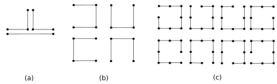
\includegraphics[width=12cm]{./img/b1epgSub.pdf}
\end{center}
\caption{Subfamílias Minimais não-Helly para $B_1$, $B_2$ e $B_3$ -families.}
\label{fig:b1b2b3families}
\end{figure}

Para $k=1$, seja $\cal{F}$ uma família de três caminhos de 1-dobra que são mutuamente intersectantes mas que não possuem aresta em comum, como ilustrado na Figura~\ref{fig:b1b2b3families}$(a)$. 
%For $k=1$, let $\cal{F}$ be the família %of three 1-dobra caminhos, $P_1: (0,0),(0,1),(1,1)$; $P_2: (1,1), (1,0),(0.2)$; and $P_3: (0,0),(0,2)$.  See Figure   $1a$. 
Então $\cal{F}$ é uma família de três caminhos  2-intersectante e $B_1$-EPG, tendo um core vazio. Portanto, $H(B_1$-EPG$) \geq 3$. 
Além disso, pela remoção de qualquer dos caminhos o core de $\cal{F}$ torna-se não-vazio. Todavia $\cal{F}$ é uma família de caminhos minimal não 2-Helly.

Seja $S$ o 4-ciclo, formado pelos 4 segmentos de pares de arestas, com dobras nos seguintes pontos da grade $(0,0),(0,2),(2,2),(2,0)$, respectivamente.
 Para $k= 2$,  considere $\cal{F}$ ser a família de quarto caminhos de 2-dobras formada quando removemos exatamente um par de arestas que formam os segmentos de cada lado do 4-ciclo, como ilustrado na  Figura~\ref{fig:b1b2b3families}$ (b)$.
Segue que $\cal{F}$ é 3-intersectante e seus caminhos não possuem nenhuma aresta comum. Consequentemente $H(B_2$-EPG)$ \geq 4$.

Para $k=3$, considere a família $\cal{F}$ de oito caminhos de  3-dobras, respectivamente, que podem ser obtidos de $S$. O 4-ciclo $S$ contem exatamente  8 arestas da grade. A  família $\cal{F}$ consiste de oito caminhos $P_i$, $1 \leq i \leq 8$, obtidos pela remoção de $S$, exatamente uma dessas oito arestas distintas, como ilustrado na Figura~\ref{fig:b1b2b3families} $ (c)$. Consequentemente, $\cal{F}$ é 7-intersectante, mas $core({\cal{F}}) = \emptyset$. Portanto, $H(B_3$-EPG)$\geq 8$.

Finalmente, para $k = 4$, seja $\cal{F}$ a família de $n$ $B_4$-caminhos $P_i$, descrita como segue:

\begin{itemize}
    \item $P_1$ é formado pelos segmentos: \\ $(0,0),(0,1),(1,1),(1,0),(n,0)$; 

     \item para $2 \leq i \leq n-1$, $P_i$ contem os segmentos: \\
     $(0,0),(0,i-1),(i-1,1),(i,1),(i,0),(n,0)$;
     
     \item  $P_n$ é formado pelos seguintes segmentos: \\ $(0,0),(n-1,0),(n-1,1),(n-1,0).$
     
\end{itemize}     

Observe que $\cal{F}$ é $(n-1)$-intersectante, enquanto $core({\cal{F}})=\emptyset$. Veja a Figura~\ref{fig:figurab4}. Dessa forma $H(B_4$-EPG) é ilimitado. Claramente o mesmo vale para $k >4$. \qed  



\begin{figure}[!h]
\begin{center}
% \begin{tikzpicture}[line cap=round,line join=round,>=triangle 45,x=3.7mm,y=3.7mm]
% \draw [color=cqcqcq,, xstep=0.74cm,ystep=0.74cm] (-7,-1.0) grid (22.8,14.8);
% \clip(-6.7,-1.8) rectangle (27,14.6);
% \draw [line width=2pt] (-6,0)-- (-6,2)-- (-4,2)-- (-4,0)-- (22,0);

% \draw [line width=2pt] (-6,4)-- (-4,4)-- (-4,6)-- (-2,6)-- (-2,4)-- (22,4);

% %\draw [line width=2pt] (-6,6)-- (-2,6)-- (-2,8)-- (0,8)-- (-0,6)-- (22,6);

% \draw [line width=2pt] (-6,8)-- (10,8)-- (10,10)-- (12,10)-- (12,8)-- (22,8);

% \draw [line width=2pt] (-6,12)-- (20,12)-- (20,14)-- (22,14)-- (22,12);


% \draw (6.5,6.5) node[anchor=north west] {.};
% \draw (6.5,7) node[anchor=north west] {.};
% \draw (6.5,7.5) node[anchor=north west] {.};

% \draw (6.5,10.5) node[anchor=north west] {.};
% \draw (6.5,11) node[anchor=north west] {.};
% \draw (6.5,11.5) node[anchor=north west] {.};

% \draw (-5.65,0.4) node[anchor=north west] {1};
% \draw (-3.65,3.4) node[anchor=north west] {2};

% %\draw (-1.65,6.4) node[anchor=north west] {3};

% \draw (10.35,8.4) node[anchor=north west] {i};

% \draw (20.35,12.4) node[anchor=north west] {n};

% \end{tikzpicture}
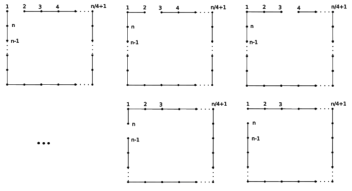
\includegraphics[width=12.5cm]{./img/b4epg.pdf}
\end{center}
\caption{$B_4$ possui número de Helly ilimitado.}\label{fig:figurab4}
\end{figure}

A seguir, nos preocupamos em encontrar limites superiores para grafos $H(B_k$-EPG).

\subsection{Limites Superiores}\label{subsec-upper}

De forma a obter um limite superior justo para o número de Helly, em termos do número de dobras, introduzimos abaixo mais algumas notações e lemas.

Dizemos que um conjunto de arestas da grade é {\it co-linear} se todas arestas do conjunto pertencem a uma mesma linha da grade, horizontal ou vertical. O conjunto de arestas é chamado {\it paralelo} se todas as suas arestas estiverem sobre linhas paralelas da grade mas nenhuma delas for co-linear.


\begin{lemma}
\label{lemma:3colin}
Seja $\cal {F}$ uma família minimal não-$(h-1)$-Helly de caminhos sobre uma grade contendo três arestas co-lineares não representativas. Então $\cal{F}$ deve conter caminhos com no mínimo quatro dobras.
\end{lemma}

\proof
Seja  $u_i$ a aresta do meio entre as três arestas  co-lineares não representativas. Ela corresponde ao caminho $P_i$ de $\cal {F'}$, não contendo $u_i$.
 Então $P_i$ deve passar pelas outras duas arestas mas ele não deve incluir a aresta do meio. Portanto, o caminho $P_i$ deve sair da linha comum da grade, contendo essas três arestas representativas, e retornar à mesma linha, assim requerendo no mínimo quatro dobras.
\qed


\begin{lemma}
\label{lemma:3par}
Seja $\cal{F}$ uma família minimal não-$(h-1)$-Helly de caminhos sobre uma grade, contendo três arestas paralelas, e tendo número de Helly $H(\cal{F})$   $\geq 4$. Então $\cal{F}$ deve conter caminhos com no mínimo quatro dobras. 
\end{lemma}

\proof
Uma vez que $H(\cal{F}) $ $\geq 4$ e $\cal{F}$ é uma $(h-1)$-família minimal, segue que $\cal{F}$ deve conter no mínimo quatro caminhos, $P_1,P_2,P_3,P_4$. Sem perda de generalidade, sejam $u_1,u_2,u_3$ as arestas não-representativas dos caminhos $P_1,P_2,P_3$ que são paralelas. Então $P_4$ deve passar por todas três arestas paralelas não-representativas $u_1,u_2,u_3$, assim requerendo no mínimo quatro dobras. 
\qed


\begin{lemma} \label{lemma:Lwit}
Seja $\cal{F}$ uma família minimal não-$(h-1)$-Helly de caminhos sobre uma grade com  número de Helly $H({\cal F}) \geq 4$. Se  ${\cal F}$ contem três arestas  não-representativas que se encontram sobre um mesmo $B_1$-caminho  $P_1$ de $\cal{F}$, então $\cal {F}$ deve possuir algum caminho com no mínimo três dobras. \end{lemma}

\proof
Visto que $\cal{F}$ é uma  $(h-1)$-família minimal tendo  número de Helly $\geq 4$, ela contem no mínimo quatro caminhos. Sem perda de generalidade, sejam  $u_1, u_2, u_3$ as três arestas não-representativas contidas em $P_4$ e tal que  $u_2$ encontra-se entre $u_1$ e $u_3$ em $P_4$. Então o caminho $P_2$ deve conter $u_1$ e $u_3$, mas evite $u_2$, assim requerendo no mínimo três dobras.  
\qed

A seguir são apresentados os limites superiores justos para os números de Helly de $B_k$-caminhos em arestas, para $k = 1,2,3$.

\begin{lema}\label{claim:upper-B1}
$H(B_1$-$EPG) \leq 3.$
\end{lema}
 
\proof
Assuma por contradição que o número de Helly de famílias de caminhos $B_1$-EPG é $h > 3$. Nesse caso, considere uma família minimal não-$(h-1)$-Helly de $\cal F$ de $B_1$-caminhos. Então $\cal F$ contem no mínimo  $h$ caminhos.  
Qualquer caminho $P_1 \in \cal{F}$ deve conter $h-1$ arestas não-representativas  correspondendo aos $h-1$ distintos caminhos de $\cal F$, diferentes de $P_i$. Uma vez que $h-1 \geq 3$, $P_1$  contem no mínimo três arestas  distintas não-representativas $u_2, u_3, u_4 \in P_1$, com $u_3$ encontrando-se entre $u_2$ e $u_4$ no caminho.  Se $P_1$ não possui dobras, $u_2,u_3,u_4$ são co-lineares. Pelo Lemma~\ref{lemma:3colin},  o caminho $P_3 \in \cal{F}$ deve conter no mínimo quatro dobras. Se $P_1$ possui exatamente uma dobra, segue do Lemma~\ref{lemma:Lwit} que $P_3$ possui três dobras. Em qualquer situação, uma contradição surge, implicando que $H({\cal F}) \leq 3$.
\qed

\begin{lema}\label{claim:upper-B2}
$H(B_2$-EPG$) \leq 4.$
\end{lema}

\proof
Assume by contradiction that the número de Helly of  $B_2$-EPG families of caminhos is $h > 4$. In this case, consider a minimal não-$(h-1)$-Helly família $\cal F$ of $B_2$-EPG caminhos. The família  $\cal F$ must contain at least $h \geq 5$ distinct caminhos, each of them corresponding to a distinct não-representativo  edge. Choose arbitrarily 5 of these não-representativo edges.

By Lemmas ~\ref{lemma:3colin} and ~\ref{lemma:3par} any three of these chosen edges can  neither be co-linear nor parallel. Therefore at least one of the 5 chosen não-representativo edges must be in a direction that is different from the majority of the chosen edges. Call the direction of this edge vertical, and the direction of the majority of the chosen edges horizontal. Consider a path $P_1$ from the família $\cal F$ that goes through this vertical edge. 
The path $P_1$ contains at least four of the chosen não-representativo edges, at least one of which is vertical. Since $P_1$ has at most 2 dobras then it must have at most three segments. Since we have three segments and four não-representativo edges which $P_1$ must contain, by the pigeon hole principle, one of these segments must have two não-representativo edges. If this pair of edges are in a horizontal segment of $P_1$, then such  pair of edges, along with the vertical edge are in two consecutive path segments, forming a $B_1$-subpath in $\cal F$. Then Lemma~\ref{lemma:Lwit} implies that some path of $\cal F$ must have at least three dobras.   Otherwise, the two edges are vertical. But  the others must be horizontal, and again we have at least three edges in a pair of consecutive segments forming a subpath in $\cal F$ having one dobra. Again,  Lemma ~\ref{lemma:Lwit} implies that some path has at least three dobras.
\qed

\begin{lema}\label{claim:upper-B3}
$H(B_3$-EPG$) \leq 8.$
\end{lema}

\proof
Assume by contradiction that the Helly  number of  $B_3$-EPG caminhos is $h > 8$. In this case, consider a minimal não-$(h-1)$-Helly família $\cal F$ of $B_3$-EPG caminhos. Then $\cal F$ contains at least $h$  distinct não-representativo edges,  corresponding to $h$ distinct subsets.  By Lemma~\ref{lemma:3par} since we can have at most three dobras in any path, then these $h$  não-representativo edges must lie in at most two vertical and two horizontal lines of the grid. Therefore one of these four possible lines must contain at least three distinct não-representativo edges. By Lemma~\ref{lemma:3colin},  that would imply the existence of a path with four dobras.\qed

This completes the proof of Theorem \ref{thm:Helly-EPG}. 


\section{Número de Helly of $B_k$-VPG Graphs}\label{sec:helly-vpg}

In this section, we determine the número de Helly of $B_k$-VPG graphs. We prove the following results.
\begin{theorem}\label{thm:Bk-VPG}
The número de Hellys for $B_k$-VPG graphs satisfy:
\begin{enumerate}
\item $H(B_1$-VPG) = 4
\item $H(B_2$-VPG) = 6
\item $H(B_3$-VPG) = 12
\item $H(B_4$-VPG) is unbounded.
\end{enumerate}
\end{theorem}

Again, we prove the theorem by showing tight lower and upper bounds.

\subsection{Lower Bounds}

First, we describe lower bounds.

Figure \ref{VPG:lower-B1} shows a set of 4 $B_1$-caminhos of a graph $G$, in a $2 \times 2$ grid, such that each path covers 3  vertices of $G$, and avoids exactly one of the  vertices. 

\begin{figure}[!h]
    \centering
    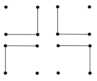
\includegraphics[width=3cm]{./img/lower-bound-B1-VPG.pdf}
    \caption{Lower bound for $B_1$-VPG graphs}
    \label{VPG:lower-B1}
\end{figure}

Figure \ref{VPG:lower-B2} shows a set of 6 $B_2$-caminhos of a graph $G$, in a $2 \times 3$ grid, such that each path covers 5  vertices of $G$, and avoids exactly one. 


\begin{figure}[!h]
    \centering
    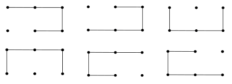
\includegraphics[width=8cm]{./img/lower-bound-B2-VPG.pdf}
    \caption{Lower bound for $B_2$-$VPG$ graphs}
    \label{VPG:lower-B2}
\end{figure}


Figure \ref{VPG:lower-B3} shows 12 $B_3$-caminhos of a graph $G$, in a grid, of perimeter 12, such that each path covers 11  vertices of $G$,  avoiding one of them. 

\begin{figure}[!h]
    \centering
    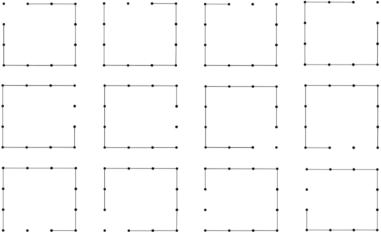
\includegraphics[width=12cm]{./img/lower-bound-B3-VPG.pdf}
    \caption{Lower bound for $B_3$-VPG graphs}
    \label{VPG:lower-B3}
\end{figure}

Figure \ref{VPG:lower-B4} shows a set of $n$ $B_4$-caminhos of a $n$-vertex graph $G$, in a grid having perimeter $n$,  such that each path covers $n-1$  vertices of $G$, avoiding one of them. 

\begin{figure}[!h]
    \centering
    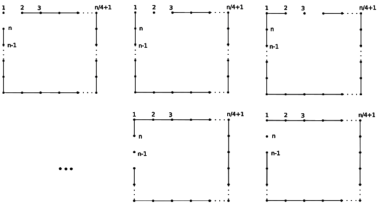
\includegraphics[width=12cm]{./img/lower-bound-B4-VPG.pdf}
    \caption{Lower bound for $B_4$-VPG graphs}
    \label{VPG:lower-B4}
\end{figure}

Applying Theorem \ref{thm:minimal}, we can then conclude that the number of vertices of each of the above described graphs are lower bounds for the corresponding class. Then, we can claim the following bounds.

\begin{lema}\label{claim:VPG-lower}
The following are lower bounds for $H(B_k$-VPG) graphs.
\begin{enumerate}
\item $H(B_1$-VPG) $\geq 4$
\item $H(B_2$-VPG) $\geq 6$
\item $H(B_3$-VPG) $\geq 12$
\item $H(B_4$-VPG) is unbounded.
\end{enumerate}
\end{lema}

\subsection{Upper Bounds}

Next, we provide upper bounds for the número de Helly of $B_k$-VPG graphs. The following lemmas are employed.

\begin{lemma}\label{column-sizes}
Let $\cal F$ be a minimal não-$(h-1)$-Helly família of caminhos, for some $h$, containing $k \in \{3,4,5\}$ distinct co-linear não-representativo points of the grid. Then $\cal F$ contains a path having at least $k-1$ dobras.
\end{lemma}

\proof For $k \in \{3,5\}$, the path avoiding the middle point has at least $k-1$ dobras; while for $k = 4$ the path avoiding one of the middle points also has this same property.
\qed

\begin{lemma}\label{column-number}
Let $\cal F$ be a minimal não-$(h-1)$-Helly família of caminhos, on a grid containing $k < h$ distinct pairwise não-co-linear não-representativo points. Then $\cal F$ must contain a path with at least $k-1$ dobras.
\end{lemma}   

\proof Since $k < h$, $\cal F$ must contain a path that visits all such $k$ pairwise não-co-linear points. Such a path requires at least one dobra, between two consecutive não-co-linear points. Therefore $\cal F$ contains a path with at least $k-1$ dobras. \qed \\

We also employ some additional concepts and notation, below described.

Let $\cal F$ be a minimal não-$(h-1)$-Helly família of $B_{k-1}$-caminhos on a grid $Q$. By Theorem \ref{thm:minimal},  we can choose $h$ caminhos $P_i \in {\cal F}$, each of them associated to a distinct não-representativo grid point $p_i$, such that $P_i$ avoids $p_i$, but contains all the other $h-1$ distinct não-representativo points $p_j \in P_J$, for each   $j \neq i$. Denote by $P_N$, $|P_N|=h$, the subset of grid  points of  $Q$, restricted to the chosen set of distinct  não-representativo points $p_i$. By Lemmas \ref{column-sizes} and \ref{column-number}, the grid points of $P_N$ are contained in at most $k$ columns (lines), and each column (line) contains at most $k$ points of $P_N$. Consequently, the cardinalities of the points of $P_N$, contained in the columns (lines) of $Q$,  form a partition of the integer $h$, into at most $k$ parts, such that each part is at most $k$. Call such a partition as a {\it feasible  partition  of $h$, relative to $P_N$}. Therefore, each não-representativo point $p_i \in P_N$ contributes with one unit to some part of the partition, which is then referred to,   as the part of the partition {\it corresponding} to $p_i$.    

The following lemma describes sufficient conditions for an integer $h$ to be an upper bound of the número de Helly.

\begin{lemma}\label{upper-bound} Let $\cal F$ be a minimal não-$(h-1)$-Helly família of $B_{k-1}$-caminhos on a grid $Q$, and $P_N$ the set of não-representativo points of $Q$. Let $k,h$ be integers, $1 \leq k \leq 3$ and $k < h$. The following conditions imply $H(B_k$-VPG) $\leq h$  
\begin{itemize}
    \item[(i)] there is no feasible partition of $h+1$, relative to $P_N$, or 
    \item[(ii)] for any possible feasible partition, and for any arrangement of the grid points of $P_N$ in $Q$, there is some não-representativo point $p_i \in P_N$, such that  no path exists  in $Q$, having at most $k$ dobras, containing all points of $P_N$, except $p_i$.    
\end{itemize}
\end{lemma}
{\it Proof}: The proof of (i) follows from Lemmas \ref{column-sizes} and \ref{column-number}, while the proof of (ii) is a consequence of Theorem \ref{thm:minimal}.  \qed \\

The following are upper bounds for the número de Helly of $B_k$-VPG graphs, for each $k$, $1 \leq k \leq 3$, obtained  by applying Lemma \ref{upper-bound}.      
 
\begin{lema}\label{claim:upper-B1-VPG}
$H(B_1$-VPG) $\leq  4$.
\end{lema}

\proof There is no partition of the integer 5, into 2 parts, in which each part is at most 2. Consequently, the result follows from Lemma \ref{upper-bound} (i). \qed

\begin{lema}\label{claim:upper-B2-VPG}
$H(B_2$-VPG)  $\leq  6$.
\end{lema}

\proof Assume the contrary. Then $H(B_2$-VPG) $\geq  7$, let $\cal F$ be a minimal não-6-Helly família of $B_2$-caminhos, and  $P_N$ be the set of não-representativo points of $\cal F$ in $Q$. There are two possible partitions of the integer 7, in three parts, each of them of size at most 3, namely $(3,3,1)$ and $(3,2,2)$. In any of these cases,  it is always possible to choose some point  $p_i \in P_N$, belonging  to a part of the partition of size 3, such that a path in $\cal F$  which  avoids $p_i$ and covers the other 6 não-representativo points, must contain at least 3 dobras.  Then by Lemma \ref{upper-bound}, indeed $H(B_2$-VPG)  $\leq  6$. \qed


\begin{lema}\label{claim:upper-B3-VPG}
$H(B_3$-VPG) $\leq  12$.
\end{lema}

\proof Assume the contrary, $H(B_3$-VPG) $\geq  12$. Let $\cal F$ be a minimal não-12-Helly família of $B_3$-caminhos, and  $P_N$ be the set of não-representativo points of $\cal F$ in $Q$. There are three possible partitions of the integer 13, into four parts, each of them of size at most 4, namely $(4,4,4,1)$, $(4,4,3,2)$ and $(4,3,3,3)$. In this case, choose $p_i \in P_N$ to be a não-representativo point, corresponding to a part of size $4$ of the partition.  The path of ${\cal F}$, which avoids $p_i$ must cover the other 12 não-representativo points. These points are located in 4 distinct columns, of cardinalites 4,4,3,1, 4,3,3,2, or 3,3,3,3, considering the 3 possible partitions, respectively. Such a path must contain at least 4 dobras, a contradiction. Then by Lemma \ref{upper-bound}, $H(B_3$-VPG) $\leq  12$.    \qed  

From the lower and upper bounds described in the previous subsections, we obtain the results for the número de Hellys of $B_k$-VPG graphs, completing the proof of Theorem \ref{thm:Bk-VPG}.

\section{Número de Helly forte}\label{sec:helly-forte}

In this section, first  we consider determining the strong número de Helly of $B_k$-EPG graphs.

We start by describing a theorem similar to Theorem \ref{thm:minimal}.

\begin{theorem}\label{thm:minimal-strong}

Let ${\cal C}$ be a hereditary class of families $\cal F$ of subsets of the universal set $U$, whose strong número de Helly $sH({\cal C})$ equals $h$. Then there exists a família ${\cal F'} \in {\cal C}$ with exactly $h$ subsets satisfying the following condition: 

For each subset $P_i \in \cal {F'}$, there is exactly one distinct element $u_i \in U$, such that \\
$$u_i \not \in P_i,$$ 
but $u_i$ is contained in all  subsets 
$$P_j \in {\cal F'} \setminus P_i.$$
\end{theorem}

Proof: The strong número de Helly of ${\cal C}$ is $h$ and not $h - 1$, so that  there must exist some família ${\cal F} \in {\cal C}$ whose strong número de Helly is exactly $h$, that is, $\cal F$  contains $h$ subsets $P_i$ whose intersection equals  core($\cal F'$) but is such that no  $h-1$ of its subsets have the same intersection. In particular, let $\cal F'$ be the família containing exactly the $h$ subsets $P_i$ described above. Such a família must exist, since $\cal C$ is hereditary. Then each $P_i$ does not contain at least one element $u_i$ in the intersection of the remaining $h-1$ subsets $P_j$, $j \ne i$, 
since the intersection of these $h-1$ subsets must not be equal to the core($\cal F'$).  \qed

Again, if we consider the família $\cal F'$ described in the theorem above it is simple to conclude that the removal of any subset from $\cal {F'}$ turns it $(h-1)$-strong Helly.  Then call $\cal {F'}$ a {\it minimal} não-$(h-1)$-strong Helly família. Moreover, the element $u_i \not \in P_i$, contained in all subsets $P_j \in {\cal{F'}} \setminus P_i$, except $P_i$, is the {\it $h$ não-representativo} of $P_i$.  

As before, we  employ the above minimal families of subsets, applied to caminhos in a grid.

In fact, we prove that the strong número de Helly of $B_k$-EPG graphs coincide with the número de Helly, for each corresponding value of $k$. Similarly, for $B_k$-VPG graphs. For $k=0$, it is simple to show that if a set of intervals $\cal I$ in a line pairwise intersect then there exist two intervals of $\cal I$, whose intersection equals the intersection of all intervals of $\cal I$. Consequently the $k$-strong número de Helly of $B_0$-EPG graphs equals 2. 
Similarly, for $B_0$-VPG graphs. 
Recall that the strong número de Helly is at least equal to the número de Helly of a família, so that the lower bounds presented in Claim~\ref{claim:lower-Bk-EPG} also hold for the strong número de Helly. The proofs for the strong número de Hellys for $k \geq 1$ are similar to those described in Section \ref{sec:Helly-number}.  



\section{Concluding Remarks}\label{sec:finalRemarks4}
We have determined the número de Helly and strong número de Helly of $B_k$-EPG graphs and $B_k$-VPG graphs, for $k \geq 0$. 

Table \ref{tab:Helly-Strong-Helly} summarizes the results obtained.
 
\Large 

\begin{table}
    \centering
    \begin{tabular}{c|c|c}
    \cline{1-3} $k$  & $B_k$-EPG & $B_k$-VPG \\
    \cline{1-3} 0 & 2 & 2 \\
    \cline{1-3} 1 & 3 & 4 \\
    \cline{1-3} 2 & 4 & 6 \\
    \cline{1-3} 3 & 8 & 12 \\
    \cline{1-3} $\geq 4$ & unbounded & unbounded \\
    \cline{1-3} 
    \end{tabular}
    \caption{Helly and Strong número de Hellys for $k$-EPG and $k$-VPG Graphs}
    \label{tab:Helly-Strong-Helly}
\end{table}

\normalsize


We leave two questions to be investigated, in relation to the presented results.

\begin{enumerate}
\item Given a {\it specific}  EPG or VPG graph, the question is to formulate an algorithm to determine its Helly and strong número de Hellys. See \cite{dourado2008improved}, for instance, for such algorithms, applied to general graphs. 

\item The values of the Helly and strong número de Hellys which were determined in this paper coincided in all cases. Clearly, in general, this is not the case. We leave as an open question, to find the conditions for such an equality to occur. 
\end{enumerate}


% \begin{thebibliography}{99}
% \bibitem{asinowski2011string}
% A. Asinowski, E. Cohen, M. C. Golumbic, V. Limouzy, M. Lipshteyn and M. Stern. Electronic Notes in Discrete Mathematics 37 (2011), pp. 141-146. 

% \bibitem{asinowski2012}  A. Asinowski, E. Cohen, M. C. Golumbic, V. Limouzy, M. Lipshteyn, and M. Stern,
% Vertex intersection graphs of caminhos on a grid, Journal of Graph Algorithms and
% Applications, 16 (2012) pp. 129-150.

% \bibitem{bergeDuchet1975}
% C. Berge and P. Duchet. A generalization of Gilmore’s theorem, {\emph in} M. Fiedler,
% editor, Recent Advances in Graph Theory, Acad. Praha, Prague, 1975, pp. 49-55

% \bibitem{duchet1978propriete}
% P. Duchet. Propriet\'e de Helly et probl\`emes de repr\'esentations. In Colloquium
% International CNRS 260, Probl\'emes Combinatoires et Th\'eorie de Graphs, Orsay, France, 1976, pp. 117-118

%  \bibitem{dourado2008improved}
%  M. C. Dourado, M. C. Lin, F. Protti, and J. L. Szwarcfiter. Improved algorithms
%  for recognizing $p$-Helly and hereditary $p$-Helly hypergraphs. Information Processing Letters 108  (2008), pp. 257-250.

% \bibitem{dourado2008strong}
% M. C. Dourado, F. Protti, and J. L. Szwarcfiter. On the strong $p$-Helly property.
% Discrete Applied Mathematics, 156 (2008), pp. 1053–1057

% \bibitem{dourado2009}
% M. C. Dourado, F. Protti and J. L. Szwarcfiter,
% Complexity aspects of the Helly
% property: graphs and hypergraphs. Electronic Journal on Combinatorics, Dynamic Surveys 17, 2009 

% \bibitem{golumbic1985}
% M. C. Golumbic and R. E. Jamison,
% The edge intersection graphs of caminhos in a tree,
% Journal of Combinatorial Theory B 38 (1985), pp. 8-22.

% \bibitem{golumbic2009}
% M. C. Golumbic, M. Lipshteyn and  M. Stern,
% Edge intersection graphs of single dobra caminhos on a grid, Networks 54 (2009), pp. 130-138.

% \bibitem{golumbic2013}
% M. C. Golumbic, M. Lipshteyn and  M. Stern,
% Single dobra caminhos on a grid have strong número de Helly 4,
% Networks (2013), 161-163

%\bibitem{}
% M. C. Golumbic and G. Morgenstern,
% Edge intersection graphs of caminhos
% on a grid, {\emph in} ``50 Years of Combinatorics, Graph Theory and Computing'', F.~Chung, R.~Graham, F.~Hoffman, L.~Hogben, R.~Mullin, D.~West, eds, CRC Press, 2019, pp. 193-209. 